\part{The Foundations of Mimetic Difference Operators 1D}

\chapter{Mathematical and Numerical Foundations of the Mimetic Difference Method}

\section{Introduction and Objectives}

\section{Notation and Prerequisites}

\begin{table}[ht!]
	\centering
	\begin{tabular}{cl}
		$\Delta x$  & tamaño de paso de la malla en la dirección $x$ \\
		$\Delta y$  & tamaño de paso de la malla en la dirección $y$ \\
		$\Delta z$  & tamaño de paso de la malla en la dirección $z$ \\
		$\symbf{D}$ & operador divergencia mimético                  \\
		$\symbf{G}$ & operador gradiente mimético                    \\
		$\symbf{L}$ & operador laplaciano mimético                   \\
		$\symbf{C}$ & operador rotacional mimético                   \\
		$\symbf{B}$ & operador frontera mimético
	\end{tabular}
\end{table}

\section{Theoretical Considerations}

\subsection{Consistency}

\subsection{Stability}

\subsection{Convergence}

\section{A Short History of Numerical Methods}

\section{Summary and Conclusions}

MOLE is an open-source library that implements high-order mimetic
operators~\cite{Corbino2024}.
Let $\Omega=\left[a,b\right]$.

\begin{align*}
	\symbf{G}f_{d}                           & =
	\vec{0}.                                     \\
	\symbf{D}\vec{v}_{d}                     & =
	0.                                           \\
	\symbf{C}\symbf{G}f                      & =
	0.                                           \\
	\symbf{D}\symbf{C}\vec{v}                & =
	0.                                           \\
	\symbf{D}\symbf{G}f_{d}                  & =
	\symbf{L}f_{d}.                              \\
	\int_{\Omega}
	f\symbf{D}\vec{v}\dl V+
	\int_{\Omega}
	\vec{v}\cdot\left(\symbf{G}f\right)\dl V & =
	\int_{\partial\Omega}
	f\vec{v}\cdot\vec{n}\dl S.                   \\
	{\left\langle
	\symbf{D}\vec{v},
	f
	\right\rangle}_{Q}+
	{\left\langle
	\symbf{G}f,
	\vec{v}
	\right\rangle}_{P}                       & =
	\left\langle
	\symbf{B}\vec{v},
	f
	\right\rangle.                               \\
	\left\langle
	Q\symbf{D}\vec{v},
	f
	\right\rangle+
	\left\langle
	P\symbf{G}f,
	\vec{v}
	\right\rangle                            & =
	\left\langle
	\symbf{B}\vec{v},
	f
	\right\rangle.                               \\
	\left\langle
	Q\symbf{D}\vec{v}+
	\symbf{G}^{T}P\vec{v},
	f
	\right\rangle                            & =
	\left\langle
	\symbf{B}\vec{v},
	f
	\right\rangle.                               \\
	Q\symbf{D}\vec{v}+
	\symbf{G}^{T}P\vec{v}                    & =
	\symbf{B}\vec{v}.                            \\
	Q\symbf{D}+
	\symbf{G}^{T}P                           & =
	\symbf{B}.
\end{align*}

\begin{equation*}
	\int_{0}^{1}
	\diff{v}{x}f\dl x+
	\int_{0}^{1}
	\diff{f}{x}\dl x=
	v\left(1\right)f\left(1\right)-
	v\left(0\right)f\left(0\right).
\end{equation*}

\begin{figure}[ht!]
	\centering
	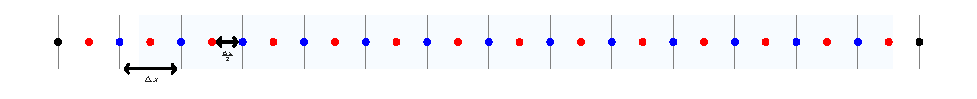
\includegraphics[width=0.8\paperwidth]{staggered}
	\caption{1D Staggered grid.}
\end{figure}

\begin{equation*}
	D^{\left(2\right)}=
	\frac{1}{h}
	\begin{bNiceMatrix}
		1 & 0 & 0 \\
		0 & 1 & 0 \\
		0 & 0 & 1
	\end{bNiceMatrix}.
\end{equation*}

\begin{equation*}
	A=
	\begin{bNiceMatrix}
		a_{11} & \cdots & a_{1c} \\
		\vdots & \ddots & \vdots \\
		a_{r1} & \cdots & a_{rc}
	\end{bNiceMatrix},
	B=
	\begin{bNiceMatrix}
		b_{11} & \cdots & b_{1q} \\
		\vdots & \ddots & \vdots \\
		b_{p1} & \cdots & a_{pq}
	\end{bNiceMatrix}
	A\otimes B\coloneqq
	\begin{bNiceMatrix}
		a_{11}B & \cdots & a_{1c}B \\
		\vdots  & \ddots & \vdots  \\
		a_{r1}B & \cdots & a_{rc}B
	\end{bNiceMatrix}.
\end{equation*}

\begin{equation*}
	D^{\left(k\right)}_{xy}=
	\begin{bNiceMatrix}
		\widehat{I}_{n}\otimes D^{\left(k\right)}_{x} &
		D^{\left(k\right)}_{y}\otimes \widehat{I}_{m}
	\end{bNiceMatrix}.
\end{equation*}

\begin{equation*}
	D^{\left(k\right)}_{xyz}=
	\begin{bNiceMatrix}
		\widehat{I}_{o}\otimes
		\widehat{I}_{n}\otimes
		D^{\left(k\right)}_{x} &
		\widehat{I}_{o}\otimes
		D^{\left(k\right)}_{y}\otimes
		\widehat{I}_{m}        &
		D^{\left(k\right)}_{z}\otimes
		\widehat{I}_{n}\otimes
		\widehat{I}_{m}        &
	\end{bNiceMatrix}.
\end{equation*}

\begin{equation*}
	G^{\left(k\right)}_{xy}=
	\begin{bNiceMatrix}
		\widehat{I}^{T}_{n}\otimes
		G^{\left(k\right)}_{x} \\
		G^{\left(k\right)}_{y}\otimes
		\widehat{I}^{T}_{m}
	\end{bNiceMatrix}.
\end{equation*}

\begin{equation*}
	G^{\left(k\right)}_{xyz}=
	\begin{bNiceMatrix}
		\widehat{I}^{T}_{o}\otimes
		\widehat{I}^{T}_{n}\otimes
		G^{\left(k\right)}_{x} \\
		\widehat{I}^{T}_{o}\otimes
		G^{\left(k\right)}_{y}\otimes
		\widehat{I}^{T}_{m}    \\
		G^{\left(k\right)}_{z}\otimes
		\widehat{I}^{T}_{n}\otimes
		\widehat{I}^{T}_{m}
	\end{bNiceMatrix}.
\end{equation*}

Compact operators

\begin{align*}
	D & =DR. \\
	G & =LG  \\
\end{align*}

\chapter{Mimetic Operadors List}

\section{Divergence 1D}

\begin{listing}[ht!]
	\tiny
	\centering
	\pathinputminted[frame=single,framesep=10pt,linenos]{octave}{div.m}
	\caption{Program~\texttt{div.m}}
	\label{code:div.m}
\end{listing}

\begin{listing}[ht!]
	\tiny
	\centering
	\pathinputminted[frame=single,framesep=10pt,linenos]{octave}{divergence.h}
	\caption{Program~\texttt{divergence.h}}
	\label{code:divergence.h}
\end{listing}

\section{Gradient 1D}

\begin{listing}[ht!]
	\tiny
	\centering
	\pathinputminted[frame=single,framesep=10pt,linenos]{octave}{grad.m}
	\caption{Program~\texttt{grad.m}}
	\label{code:grad.m}
\end{listing}

\begin{listing}[ht!]
	\tiny
	\centering
	\pathinputminted[frame=single,framesep=10pt,linenos]{octave}{gradient.h}
	\caption{Program~\texttt{gradient.h}}
	\label{code:gradient.h}
\end{listing}

\section{Laplacian 1D}

\begin{listing}[ht!]
	\tiny
	\centering
	\pathinputminted[frame=single,framesep=10pt,linenos]{octave}{lap.m}
	\caption{Program~\texttt{lap.m}}
	\label{code:lap.m}
\end{listing}

\begin{listing}[ht!]
	\tiny
	\centering
	\pathinputminted[frame=single,framesep=10pt,linenos]{octave}{laplacian.h}
	\caption{Program~\texttt{laplacian.h}}
	\label{code:laplacian.h}
\end{listing}

\section{Interpolation 1D}

\begin{listing}[ht!]
	\tiny
	\centering
	\pathinputminted[frame=single,framesep=10pt,linenos]{octave}{interpol.m}
	\caption{Program~\texttt{interpol.m}}
	\label{code:interpol.m}
\end{listing}

\section{Divergence 2D}

\begin{listing}[ht!]
	\tiny
	\centering
	\pathinputminted[frame=single,framesep=10pt,linenos]{octave}{div2D.m}
	\caption{Program~\texttt{div2D.m}}
	\label{code:div2D.m}
\end{listing}

\section{Gradient 2D}

\begin{listing}[ht!]
	\tiny
	\centering
	\pathinputminted[frame=single,framesep=10pt,linenos]{octave}{grad2D.m}
	\caption{Program~\texttt{grad2D.m}}
	\label{code:grad2D.m}
\end{listing}

\section{Laplacian 2D}

\begin{listing}[ht!]
	\tiny
	\centering
	\pathinputminted[frame=single,framesep=10pt,linenos]{octave}{lap2D.m}
	\caption{Program~\texttt{lap2D.m}}
	\label{code:lap2D.m}
\end{listing}

\section{Interpolation 2D}

\begin{listing}[ht!]
	\tiny
	\centering
	\pathinputminted[frame=single,framesep=10pt,linenos]{octave}{interpol2D.m}
	\caption{Program~\texttt{interpol2D.m}}
	\label{code:interpol2D.m}
\end{listing}

\section{Divergence 3D}

\begin{listing}[ht!]
	\tiny
	\centering
	\pathinputminted[frame=single,framesep=10pt,linenos]{octave}{div3D.m}
	\caption{Program~\texttt{div3D.m}}
	\label{code:div3D.m}
\end{listing}

\section{Gradient 3D}

\begin{listing}[ht!]
	\tiny
	\centering
	\pathinputminted[frame=single,framesep=10pt,linenos]{octave}{grad3D.m}
	\caption{Program~\texttt{grad3D.m}}
	\label{code:grad3D.m}
\end{listing}

\section{Laplacian 3D}

\begin{listing}[ht!]
	\tiny
	\centering
	\pathinputminted[frame=single,framesep=10pt,linenos]{octave}{lap3D.m}
	\caption{Program~\texttt{lap3D.m}}
	\label{code:lap3D.m}
\end{listing}

\section{Interpolation 3D}

\begin{listing}[ht!]
	\tiny
	\centering
	\pathinputminted[frame=single,framesep=10pt,linenos]{octave}{interpol3D.m}
	\caption{Program~\texttt{interpol3D.m}}
	\label{code:interpol3D.m}
\end{listing}

\section{Interpolation 1D from center to nodes}

\section{Interpolation 2D from center to nodes}

\section{Interpolation 3D from center to nodes}

\section{Interpolation 1D from center to faces}

% interpolCentersToFacesD1D.m

\section{Interpolation 2D from center to faces}

\section{Interpolation 3D from center to faces}

\section{Interpolation 1D from nodes to center}

\section{Interpolation 2D from nodes to center}

\section{Interpolation 3D from nodes to center}

\section{Interpolation 1D from faces to center}

\section{Interpolation 2D from faces to center}

\section{Interpolation 3D from faces to center}

\section{Add Boundary Conditions 1D}

\begin{listing}[ht!]
	\tiny
	\centering
	\pathinputminted[frame=single,framesep=10pt,linenos]{octave}{addBC1D.m}
	\caption{Program~\texttt{addBC1D.m}}
	\label{code:addBC1D.m}
\end{listing}


Let be
\begin{math}
	f,g\colon\Omega\subset\mathbb{R}^{n}\to
	\mathbb{R}
\end{math}
are scalar fields.
Let be
\begin{math}
	\vec{v},\vec{w}\colon\Omega\subset\mathbb{R}^{n}\to
	\mathbb{R}^{m}
\end{math}
are vector fields.

\begin{align*}
	\left\langle
	f,g
	\right\rangle & =
	\int_{\Omega}fg \dl V. \\
	\left\langle
	\vec{v},\vec{w}
	\right\rangle & =
	\int_{\Omega}\vec{v}\vec{w}\dl V.
\end{align*}

\begin{align*}
	\left\langle
	\symbf{D}\vec{v},
	f
	\right\rangle+
	\left\langle
	\vec{v},
	\symbf{G}f
	\right\rangle & =
	\int_{\partial\Omega}
	f\vec{v}\cdot\vec{n}\dl S.
\end{align*}

\begin{align*}
	\symbf{G}\colon\mathbb{R}^{n+2} & \longrightarrow
	\mathbb{R}^{n+1}                                  \\
	f                               & \longmapsto
	\symbf{G}f.
\end{align*}

\begin{align*}
	\symbf{D}\colon\mathbb{R}^{n+1} & \longrightarrow
	\mathbb{R}^{n}                                    \\
	\vec{v}                         & \longmapsto
	\symbf{D}\vec{v}.
\end{align*}

\begin{align*}
	\symbf{B}\colon\mathbb{R}^{n+2} & \longrightarrow
	\mathbb{R}^{n+1}                                  \\
	\vec{v}                         & \longmapsto
	\symbf{B}\vec{v}.
\end{align*}

\begin{theorem}{}{}
	Let be
	\begin{math}
		f=
		\begin{bNiceMatrix}
			f_{0}             &
			f_{\frac{1}{2}}   &
			f_{\frac{3}{2}}   &
			\cdots            &
			f_{n-\frac{1}{2}} &
			f_{n}
		\end{bNiceMatrix}^{T}\in\mathbb{R}^{n+2}
	\end{math}
	a discretized function defined at the cell centers and
	at the boundary of the 1D mesh.
	Let be
	\begin{math}
		v=
		\begin{bNiceMatrix}
			v_{0}  &
			v_{1}  &
			\cdots &
			v_{n}
		\end{bNiceMatrix}^{T}\in\mathbb{R}^{n+1}
	\end{math}
	a discretized function defined on the nodes of the 1D mesh.

	\begin{itemize}
		\item

		      \begin{math}
			      \symbf{G}f=
			      0\iff f=
			      c
		      \end{math}.

		\item

		      \begin{math}
			      \symbf{D}\vec{v}=
			      0\iff\vec{v}=
			      c
		      \end{math}.
	\end{itemize}
\end{theorem}

\begin{proof}\leavevmode
	\begin{itemize}
		\item

		      \begin{align*}
			      \symbf{D}\vec{v} & =
			      \frac{v_{i+1}-v_{i}}{\Delta x}. \\
			      0                & =
			      \frac{v_{i+1}-v_{i}}{\Delta x}.
		      \end{align*}

		\item

		      \begin{align*}
			      \symbf{G}f & =
			      \frac{f_{i+\frac{1}{2}}-f_{i-\frac{1}{2}}}{\Delta x}.
		      \end{align*}
	\end{itemize}
\end{proof}

\begin{equation*}
	\symbf{G}_{x}u=
	\symbf{G}u\left(x_{i},y_{j+\frac{1}{2}}\right)=
	\symbf{G}_{i,j+\frac{1}{2}}.
\end{equation*}

\begin{equation*}
	\symbf{G}_{y}u=
	\symbf{G}u\left(x_{i+\frac{1}{2}},y_{j}\right)=
	\symbf{G}_{i+\frac{1}{2},j}.
\end{equation*}

\begin{equation*}
	\symbf{D}_{\vec{v}}\left(x_{i+\frac{1}{2}},y_{j+\frac{1}{2}}\right)=
	\symbf{D}\vec{v}_{i+\frac{1}{2},j+\frac{1}{2}}.
\end{equation*}

\chapter{Numerical Methods for Differential Equations}

\section{Ordinary Differential Equations (ODEs)}

\subsection{Initial Value Problems}

\todo{Only the methods used in the tutorials: Verlett, RK4, Explicit Euler}

Consider the Initial Value Problem

\begin{equation*}
	\begin{cases}
		\diff{y}{t}=
		f\left(t,y\right), & t\in\left[0,T\right]. \\
		y\left(0\right)=
		y_{0}.             &
	\end{cases}
\end{equation*}

\subsubsection{Backward Euler Method}
% https://www.youtube.com/watch?v=HeVsOss1w78
\begin{equation*}
	f\left(t_{n+1},y_{n+1}\right)
	=\diff{y}{t}\approx
	\frac{y_{n+1}-y_{n}}{\Delta t}\implies
	y_{n+1}=
	y_{n}+
	f\left(t_{n+1},y_{n+1}\right)
	\Delta t.
\end{equation*}

The local truncation error is
\begin{math}
	\mathcal{O}
	\left(\Delta t^{2}\right)
\end{math}.
The Butcher table is
\begin{math}
	\renewcommand\arraystretch{1.2}
	\begin{array}
		{c|c}
		1 & 1 \\
		\hline
		  & 1
	\end{array}
\end{math}.

\begin{equation*}
	\begin{cases}
		\diff{y}{t}=
		y\sin t^{2},       & t\in\left[0,5\right]. \\
		y\left(0\right)=2. &
	\end{cases}
\end{equation*}

\begin{equation*}
	S\left(x\right)\coloneqq
	\int_{0}^{x}\sin\left(t^{2}\right)\dl t=
	\sum_{n=0}^{\infty}
	\frac{{\left(-1\right)}^{n}x^{4n+3}}{\left(2n+1\right)!\left(4n+3\right)}.
\end{equation*}

We integrate and obtain the general solution.
\begin{align*}
	\iint
	\diff[2]{u}{x}
	\dl x
	\dl x           & =
	\iint
	e^{x}
	\dl x
	\dl x.              \\
	\int
	\diff{u}{x}
	\dl x           & =
	\int
	\left(e^{x}+C_{1}\right)
	\dl x.              \\
	u\left(x\right) & =
	e^{x}+C_{1}x+C_{2}.
\end{align*}
Now, let's apply the Robin boundary conditions.
\begin{equation}\label{eq:linearsystem}
	\left\{
	\begin{aligned}
		0
		 & =
		u\left(0\right)-
		\diff{u}{x}[x=0]=
		e^{0}+C_{1}\left(0\right)+C_{2}-
		\left(e^{0}+C_{1}\right)=
		C_{2}-C_{1}. \\
		2e
		 & =
		u\left(1\right)+
		\diff{u}{x}[x=1]=
		e^{1}+C_{1}\left(1\right)+C_{2}+
		\left(e^{1}+C_{1}\right)=
		2e+2C_{1}+C_{2}.
	\end{aligned}
	\right.
\end{equation}
El sistema~\eqref{eq:linearsystem} tiene como solución
$C_{1}=C_{2}=0$.
$\therefore$ la solución
de~\eqref{eq:poisson1drobindconditions} es
$u\left(x\right)=e^{x}$.

\begin{listing}[ht!]
	\tiny
	\centering
	\pathinputminted[frame=single,framesep=10pt,linenos,firstline=1,lastline=13,highlightlines={12}]{octave}{backward_euler.m}
	\caption{Program~\texttt{backward\_euler.m}}
	\label{code:backward_euler.m}
\end{listing}

\begin{figure}[ht!]
	\centering
	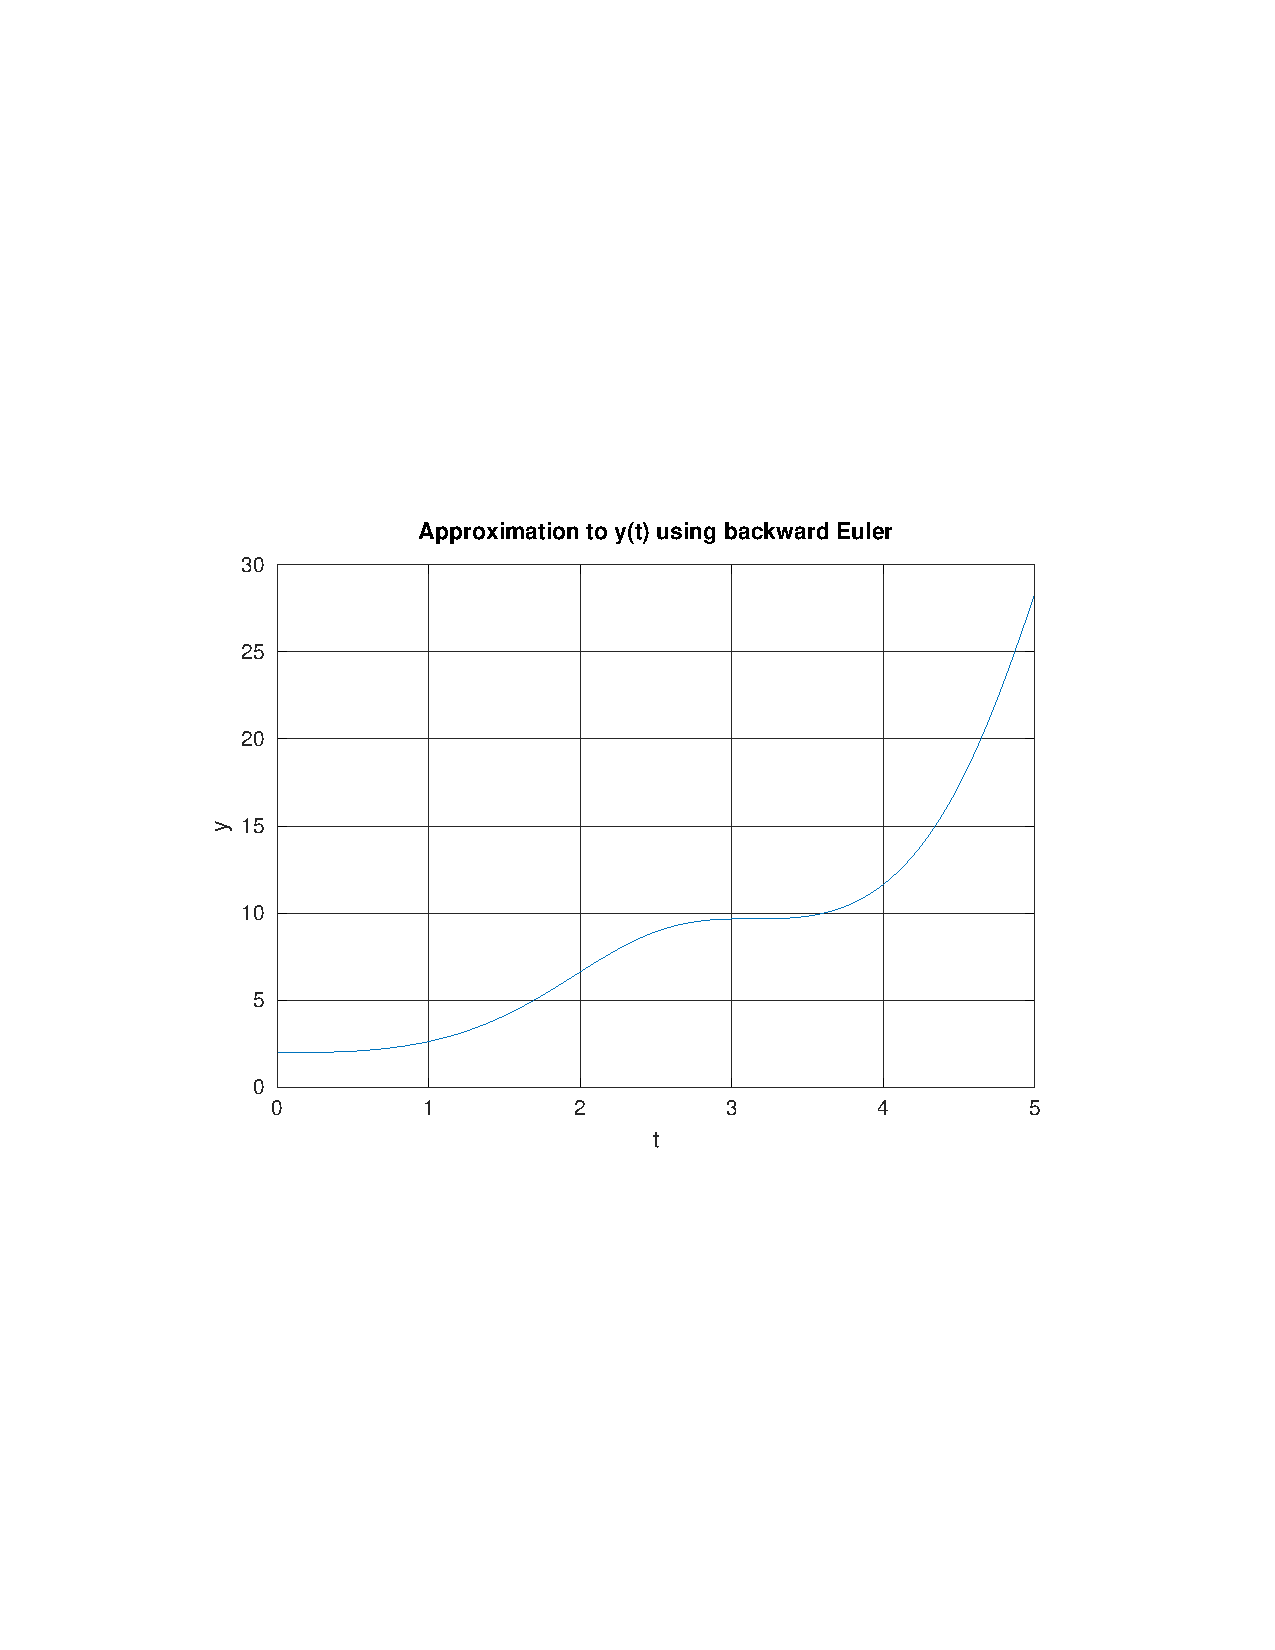
\includegraphics[width=0.55\paperwidth]{backward_euler.pdf}
	\caption{Numerical solution by the Backward Euler Method.}
\end{figure}

\begin{itemize}
	\item

	      \url{https://docs.octave.org/v9.4.0/Ranges.html}

	\item

	      \url{https://docs.octave.org/v9.4.0/Solvers.html#XREFfzero}

	\item

	      \url{https://docs.octave.org/v9.4.0/Object-Sizes.html#XREFsize}

	\item

	      \url{https://docs.octave.org/v9.4.0/Object-Sizes.html#XREFlength}

	\item

	      \url{https://docs.octave.org/v9.4.0/Trigonometry.html#XREFsin}

	\item

	      \url{https://docs.octave.org/v9.4.0/Special-Utility-Matrices.html#XREFzeros}
\end{itemize}

% \url{https://docs.octave.org/v9.4.0/Basic-Vectorization.html}
% \url{https://docs.octave.org/v9.4.0/Ordinary-Differential-Equations.html}

\subsubsection{Explicit Runge-Kutta 2}
% https://www.youtube.com/watch?v=HeVsOss1w78
\begin{align*}
	\widetilde{y}_{n+1} & =
	y_{n}+
	f\left(t_{n},y_{n}\right)\Delta t. \\
	y_{n+1}             & =
	y_{n}+
	\frac{\Delta t}{2}
	\left(
	f\left(t_{n},y_{n}\right)+
	f\left(\widetilde{y}_{n+1},t_{n+1}\right)
	\right).
\end{align*}

The local truncation error is
\begin{math}
	\mathcal{O}
	\left(\Delta t^{2}\right)
\end{math}.
The Butcher table is
\begin{math}
	\renewcommand\arraystretch{1.2}
	\begin{array}
		{c|cc}
		0 &             &             \\
		1 & 1           &             \\
		\hline
		  & \frac{1}{2} & \frac{1}{2}
	\end{array}
\end{math}.

\begin{listing}[ht!]
	\tiny
	\centering
	\pathinputminted[frame=single,framesep=10pt,linenos,firstline=1,lastline=14,highlightlines={11-13}]{octave}{RK2.m}
	\caption{Program~\texttt{RK2.m}}
	\label{code:RK2.m}
\end{listing}

\begin{listing}[ht!]
	\tiny
	\centering
	\pathinputminted[frame=single,framesep=10pt,linenos,firstline=1,lastline=81,highlightlines={41-47}]{cpp}{RK2.cpp}
	\caption{Program~\texttt{RK2.cpp}}
	\label{code:RK2.cpp}
\end{listing}

\begin{figure}[ht!]
	\centering
	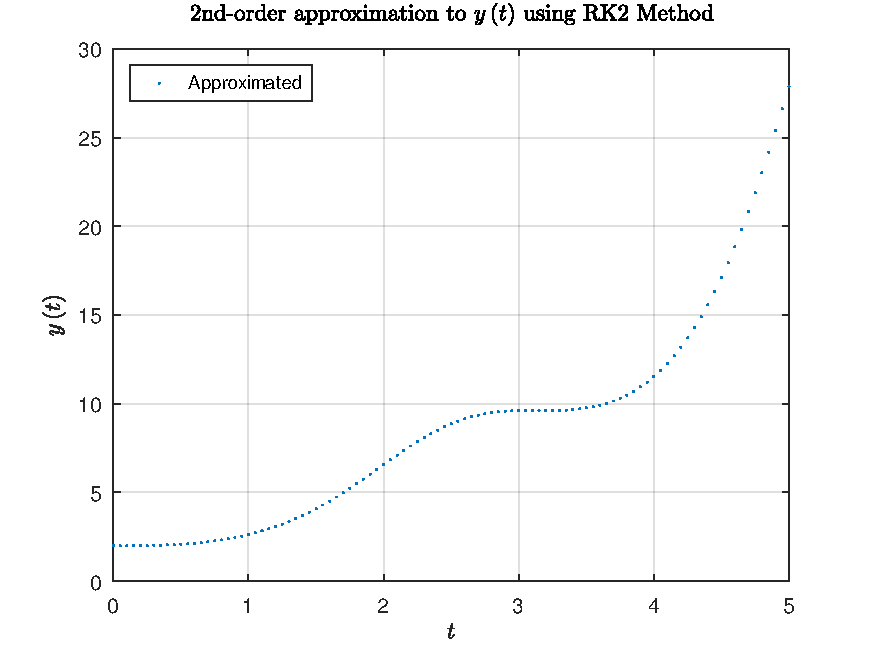
\includegraphics[width=0.55\paperwidth]{RK2.pdf}
	\caption{Numerical solution by the Runge-Kutta 2 Method.}
\end{figure}

\subsubsection{Explicit Runge-Kutta 4}
% https://jonshiach.github.io/ODEs-book/_pages/2.3_RK4_Derivation.html
% https://www.youtube.com/watch?v=qUe_kR7QoBU

\begin{align*}
	k_{1}   & =
	f\left(t_{n},y_{n}\right).                                            \\
	k_{2}   & =
	f\left(t_{n}+\frac{\Delta t}{2},y_{n}+\Delta t\frac{k_{1}}{2}\right). \\
	k_{3}   & =
	f\left(t_{n}+\frac{\Delta t}{2},y_{n}+\frac{\Delta k_{2}}{2}\right).  \\
	k_{4}   & =
	f\left(t_{n}+\Delta t,y_{n}+\Delta t k_{3}\right).                    \\
	y_{n+1} & =
	y_{n}+
	\frac{1}{6}\left(k_{1}+2k_{2}+2k_{3}+k_{4}\right).
\end{align*}

The local truncation error is
\begin{math}
	\mathcal{O}
	\left(\Delta t^{4}\right)
\end{math}.
The Butcher table is
\begin{math}
	\renewcommand\arraystretch{1.2}
	\begin{array}
		{c|cccc}
		0           &             &             &             &             \\
		\frac{1}{2} & \frac{1}{2} &             &             &             \\
		\frac{1}{2} & 0           & \frac{1}{2} &             &             \\
		1           & 0           & 0           & 1           &             \\
		\hline
		            & \frac{1}{6} & \frac{4}{6} & \frac{4}{6} & \frac{1}{6}
	\end{array}
\end{math}.

\begin{listing}[ht!]
	\tiny
	\centering
	\pathinputminted[frame=single,framesep=10pt,linenos,firstline=1,lastline=16,highlightlines={11-15}]{octave}{RK4.m}
	\caption{Program~\texttt{RK4.m}}
	\label{code:RK2.m}
\end{listing}

\begin{figure}[ht!]
	\centering
	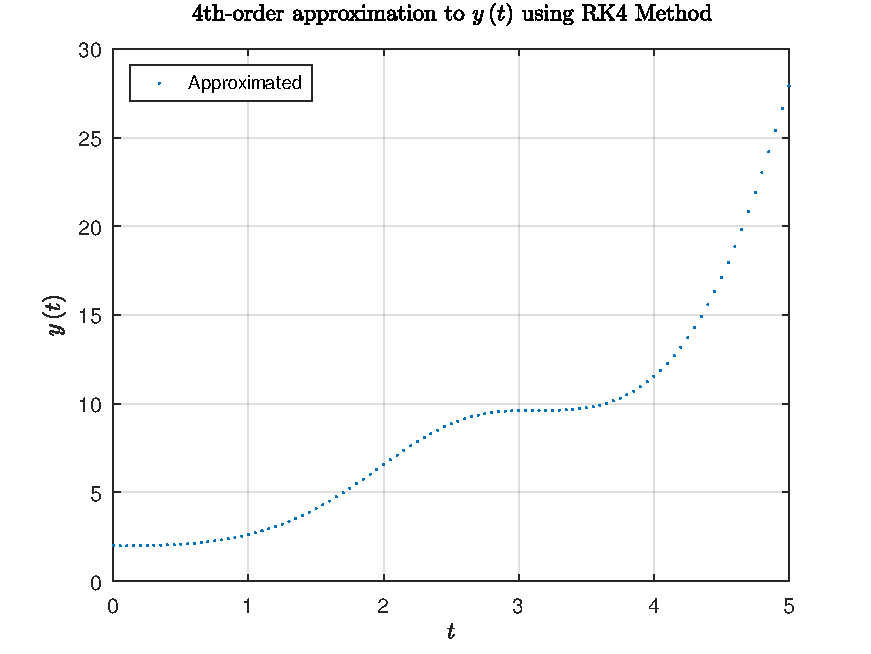
\includegraphics[width=0.55\paperwidth]{RK4.pdf}
	\caption{Numerical solution by the Runge-Kutta 4 Method.}
\end{figure}

\subsubsection{Verlett}

\subsection{Boundary Value Problems}

\section{Partial Differential Equations (PDEs)}

\subsection{Hyperbolic Equation (transport)}

\subsection{Parabolic Equation (Diffusion)}

\subsection{Elliptic Equation (Poisson)}

\subsubsection{von Neumann Stability Analysis}

\subsubsection{Convergence and Error Estimation}

